%!TEX encoding = UTF-8 Unicode
%!TEX program = xelatex

\documentclass[bachelor]{ustcthesis}
% bachelor|master|doctor
\usepackage{ustcextra}
\graphicspath{{figures/}}
\bibliographystyle{ustcauthoryear}
% \bibliographystyle{ustcnumerical}

\renewpagestyle{front}[\zihao{-5}]{
    \sethead{}{软件工程作业管理系统概要设计}{}
    \setfoot{}{\thepage}{}
    \headrule
}
\renewpagestyle{main}[\zihao{-5}]{
    \sethead{}{软件工程作业管理系统概要设计}{}
    \setfoot{}{\thepage}{}
    \headrule
}
\newcommand{\HRule}{\rule{\linewidth}{0.5mm}}
\newcommand{\tabincell}[2]{\begin{tabular}{@{}#1@{}}#2\end{tabular}}

\begin{document}



\begin{titlepage}
\begin{center}
~\\[5cm]
\HRule \\[0.4cm]
{\huge \bfseries 软件工程作业管理系统\\概要设计}\\[0.4cm]
\HRule \\[1.5cm]

\begin{tabular}{ccc}
  & 人员 & 日期 \\ 
拟制 & 张三\ 李四\ 王五 & yyyy-mm-dd \\ 
评审人 & • & yyyy-mm-dd \\ 
批准 & • & yyyy-mm-dd \\ 
签发 & • & yyyy-mm-dd \\ 
\end{tabular} 

\end{center}
\end{titlepage}



\frontmatter
\begin{abstract}
ETS 考试与管理系统是由 ETS 投资开发,以实现 TOFEL、GRE、GMAT 考试网络化、信息化,高效为考生服务的重要工作之一。该系统是一个新的独立的项目。它充分考虑了考生的需求,利用网络的便捷性,提高考生获取信息的能力,方便了考试流程。同时该系统也方便了 ETS 管理人员进行试题、成绩等数据的管理。本系统可以与其他应用系统交互,极大的增强了交互性和可操作性。

本文档是该软件工程的概要设计,包括接口设计、数据结构设计、数据库设计等。此外还包含了维护与安全性等内容。

\keywords{软件工程\zhspace{} 概要设计\zhspace{} ETS考试与管理系统\zhspace{}}

\begin{table}[htbp]
\centering
\caption{缩略词清单} \label{tab:simpletable}
\begin{tabular}{|c|c|c|}
    \hline
    缩略语 & 英文全名 & 中文解释 \\
    \hline
    DB & database & 数据库 \\
    \hline
    ER model & Entity-Relation model & 实体-关系模型 \\
    \hline
    ADO & ActiveX Data Object & 一个com组件,用于访问连接数据库 \\
    \hline
    UI & User Interface & 用户界面 \\
    \hline
\end{tabular}
\end{table}

\end{abstract}

\tableofcontents
\listoffigures
\listoftables
% \listofalgorithms  % 算法索引,如不需要,可直接注释掉本行
% \begin{notation}

%\centering
%XX 软件需求规格说明书

%关键词:能够体现文档描述内容主要方面的词汇。
 
%摘要:


\centering
\begin{tabular}{rl}
$\ln x$ & natural logarithm $\log_ex$ \\
$\log x$ & common logarithm $\log_{10}x$ \\
$x\ \mathrm{mod}\ y$ & remainder \\
\end{tabular}

\end{notation}


\mainmatter
\chapter{引言}
\section{编写目的}
在本项目的前一阶段,也就是需求分析阶段,已经将系统用户对本系统的需求做了详细的阐述,这些用户需求已经在上一阶段中对不同用户所提出的不同功能,实现的各种效果做了调研工作,并在需求规格说明书中得到详尽得叙述及阐明。

本阶段已在系统的需求分析的基础上,对即时聊天工具做概要设计。主要解决了实现该系统需求的程序模块设计问题。包括如何把该系统划分成若干个模块、决定各个模块之间的接口、模块之间传递的信息,以及数据结构、模块结构的设计等。在以下的概要设计报告中将对在本阶段中对系统所做的所有概要设计进行详细的说明,在设计过程中起到了提纲挈领的作用。

在下一阶段的详细设计中,程序设计员可参考此概要设计报告,在概要设计即时聊天工具所做的模块结构设计的基础上,对系统进行详细设计。在以后的软件测试以及软件维护阶段也可参考此说明书,以便于了解在概要设计过程中所完成的各模块设计结构,或在修改时找出在本阶段设计的不足或错误。


\section{项目背景}
随着xxx的不断发展...

\section{术语}
[列出本文档中所用到的专门术语的定义和外文缩写的原词组]
\begin{table}[htbp]
\centering
\caption{术语表} \label{tab:terminology}
\begin{tabular}{|c|c|}
    \hline
    缩写、术语 & 解释 \\
    \hline
    c & d \\
    \hline
\end{tabular}
% \note{这里是表的注释}
\end{table}
\chapter{任务概述}
本系统的目标是实现一个ETS考试与管理系统,包括客户端、服务器端两个部分。

客户端面向考生用户,为用户提供账号注册、考位查询、缴费、考试报名、成绩查询等服务。
服务器端面向ETS管理员用户,为用户提供考试信息发布、题库维护、试题发布、试卷分发及测试、试卷批改等服务。

\section{目标}
实现ETS考试与管理系统,实现需求规格说明书中所描述的面向考生用户和面向ETS管理员用户的各个功能,并且保证系统的健壮性和数据安全。

\section{开发与运行环境}

\subsection{开发环境的配置}
\begin{table}[htbp]
\centering
\caption{开发环境的配置} \label{tab:development-environment}
\begin{tabular}{|c|c|c|}
    \hline
    类别 & 标准配置 & 最低配置 \\
    \hline
    计算机硬件 & \tabincell{c}{因特尔 Xeon 5335 2颗\\ 主频 2.0GHz\\ 2G FBD内存 4条\\ 146GSAS 15000转硬盘 2 RAID 1级别容错} & \tabincell{c}{因特尔 Xeon 5405 1颗\\ 主频 2.0GHz\\ 1G FBD667内存 2条\\ 250G SATA硬盘 2 RAID 1级别容错} \\
    \hline
    计算机软件 & \tabincell{c}{微软 Windows Server 2016\\ Microsoft Visual C++ 2015} & \tabincell{c}{微软 Windows Server 2016\\ Microsoft Visual C++ 2015} \\
    \hline
    网络通信 & \tabincell{c}{思科WMP600N 300m 双频 PCI无线网卡\\ 能运行IP协议栈} & \tabincell{c}{思科AE1200 AE2500双频USB无线网卡\\ 能运行IP协议栈} \\
    \hline
    数据库 & Oracle Database 12c 企业版 & Oracle Database 12c 企业版 \\
    \hline
\end{tabular}
% \note{这里是表的注释}
\end{table}

\subsection{测试环境的配置}
\begin{table}[htbp]
\centering
\caption{测试环境的配置} \label{tab:test-environment}
\begin{tabular}{|c|c|c|}
    \hline
    类别 & 标准配置 & 最低配置 \\
    \hline
    计算机硬件 & \tabincell{c}{因特尔 Xeon 5335 2颗\\ 主频 2.0GHz\\ 2G FBD内存 4条\\ 146GSAS 15000转硬盘 2 RAID 1级别容错} & \tabincell{c}{因特尔 Xeon 5405 1颗\\ 主频 2.0GHz\\ 1G FBD667内存 2条\\ 250G SATA硬盘 2 RAID 1级别容错} \\
    \hline
    计算机软件 & \tabincell{c}{微软 Windows Server 2016\\ Microsoft Visual C++ 2015} & \tabincell{c}{微软 Windows Server 2016\\ Microsoft Visual C++ 2015} \\
    \hline
    网络通信 & \tabincell{c}{思科WMP600N 300m 双频 PCI无线网卡\\ 能运行IP协议栈} & \tabincell{c}{思科AE1200 AE2500双频USB无线网卡\\ 能运行IP协议栈} \\
    \hline
    数据库 & Oracle Database 12c 企业版 & Oracle Database 12c 企业版 \\
    \hline

\end{tabular}
% \note{这里是表的注释}
\end{table}

\subsection{运行环境的配置}
\begin{table}[htbp]
\centering
\caption{运行环境的配置} \label{tab:operation-environment}
\begin{tabular}{|c|c|c|}
    \hline
    类别 & 标准配置 & 最低配置 \\
    \hline
    计算机硬件 & \tabincell{c}{因特尔 Xeon 5335 2颗\\ 主频 2.0GHz\\ 2G FBD内存 4条\\ 146GSAS 15000转硬盘 2 RAID 1级别容错} & \tabincell{c}{因特尔 Xeon 5405 1颗\\ 主频 2.0GHz\\ 1G FBD667内存 2条\\ 250G SATA硬盘 2 RAID 1级别容错} \\
    \hline
    计算机软件 & \tabincell{c}{微软 Windows Server 2016\\ Microsoft Visual C++ 2015} & \tabincell{c}{微软 Windows Server 2016\\ Microsoft Visual C++ 2015} \\
    \hline
    网络通信 & \tabincell{c}{思科WMP600N 300m 双频 PCI无线网卡\\ 能运行IP协议栈} & \tabincell{c}{思科AE1200 AE2500双频USB无线网卡\\ 能运行IP协议栈} \\
    \hline
    数据库 & Oracle Database 12c 企业版 & Oracle Database 12c 企业版 \\
    \hline

\end{tabular}
% \note{这里是表的注释}
\end{table}

\section{需求概述}
功能需求包括:

供考生使用的客户端系统提供的功能:新用户注册、个人信息管理、考试时间地点考位查询、考试报名、成绩查询。

供ETS管理员使用的服务器端系统提供的功能有:考试信息发布、题库维护、试题成型、试卷分发及测试、试卷批改。


\section{条件与限制}
本系统使用的技术约束如下:

编程语言:

1、前端:HTML+CSS+Javascript

2、后端:C++

接口:

1、操作系统:服务器端:Windows Server 2016,客户端:支持浏览器的主流操作系统(Windows 7/8/8.1/10, Ubuntu等)
	
2、数据库:Oracle Database 12c 企业版
	
3、集成开发环境:Visual Studio 2015
	
4、库:ADO
	
5、通信:浏览器(HTTPS)
	
6、编程规范:参见《ETS考试报名、缴费与考场管理系统开发编程规范》中的具体说明。


\chapter{总体设计}
\section{软件描述}
系统包括考生用户子系统和ETS管理子系统两个部分。

考生子系统的主要功能是为考生用户提供以下服务:

1、注册成为系统的新用户

2、查询、更改自己的个人信息

3、查询考试时间、地点、考位信息

4、考试报名与取消报名

5、成绩查询

ETS管理子系统的主要功能是:

1、考试信息发布

2、题库维护

3、试题成型

4、试卷分发及测试

5、试卷批改

\section{处理流程}
\subsection{总体流程}

\subsection{系统基本流程}
\begin{figure}[ht]
\centering
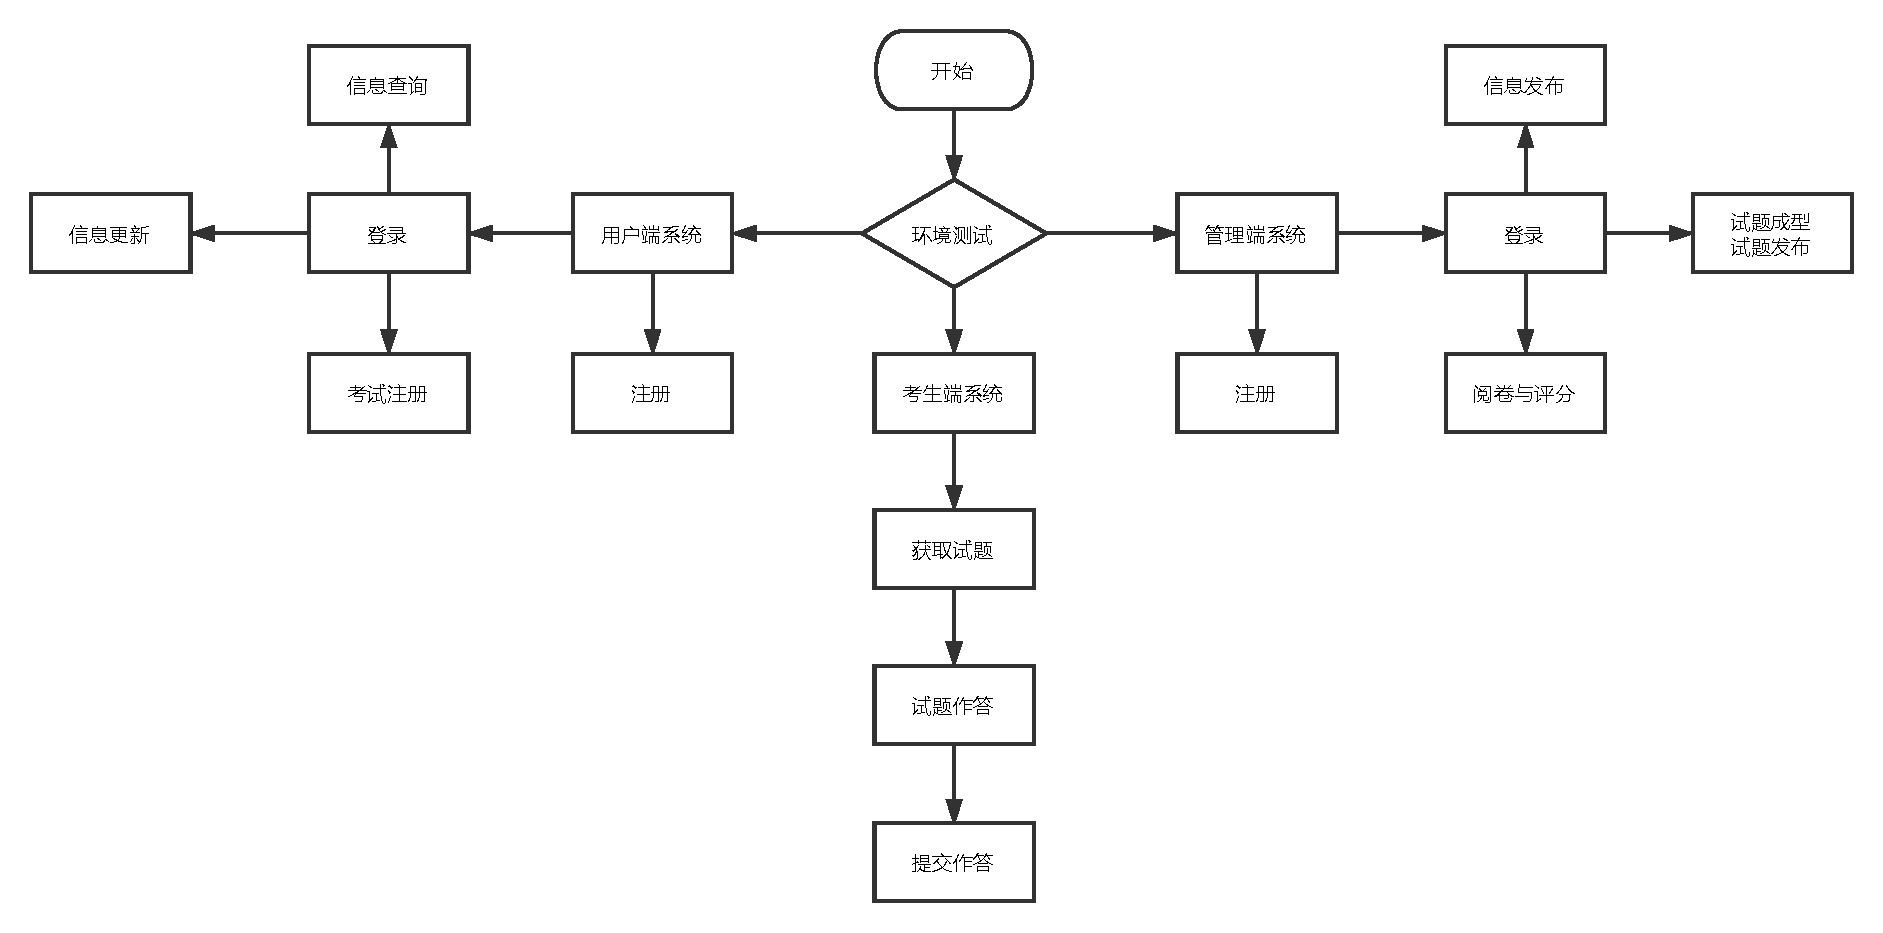
\includegraphics[width=10cm]{basic}
\caption{系统基本流程} \label{fig:figure1}
\end{figure}

用户先注册,向ETS系统提交其相关的个人信息,然后通过其用户名与密码登陆,进行后续操作。在登陆界面,用户可以查询个人信息、更新个人信息、查询并注册考试等。管理员同样需要进行受限的注册与登陆操作,然后可以进行考试信息发布、题目添加、试题成型、试卷分发、阅卷等操作。

\subsection{客户端基本流程}
\begin{figure}[ht]
\centering
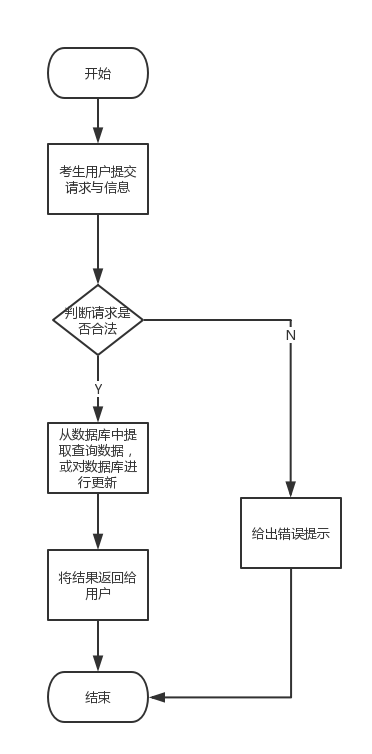
\includegraphics[width=10cm]{flowchart1.png}
\caption{考生用户子系统总体流程} \label{fig:figure1}
\end{figure}

上图是考生用户子系统总体流程图。系统接受用户的请求及附带的用户提供的信息,检测这些请求是否符合用户所具有的权限,以及检测用户所提交的信息是否符合要求。如果检测通过,则按照用户请求对数据库进行相应的增删改查等操作,并将操作结果返回给用户。否则,拒绝请求,并返回错误信息。

\subsection{服务器端基本流程}
\begin{figure}[ht]
\centering
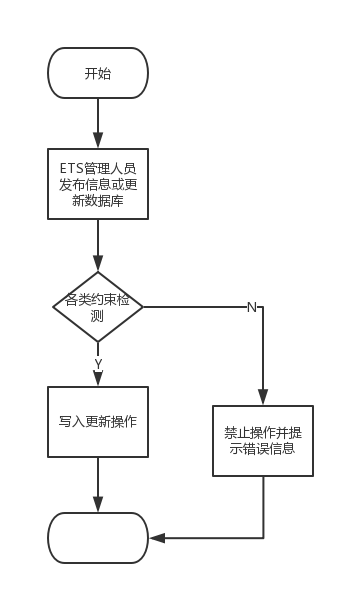
\includegraphics[width=10cm]{flowchart2.png}
\caption{ETS管理子系统总体流程} \label{fig:figure1}
\end{figure}

上图是ETS管理子系统总体流程图。系统接受用户提交的各类请求,验证用户身份及其所具有的权限,并进行完整性检查。如果检查通过,执行用户请求的操作。否则,拒绝操作并给出错误信息。

\subsection{注册功能具体流程}
\begin{figure}[ht]
\centering
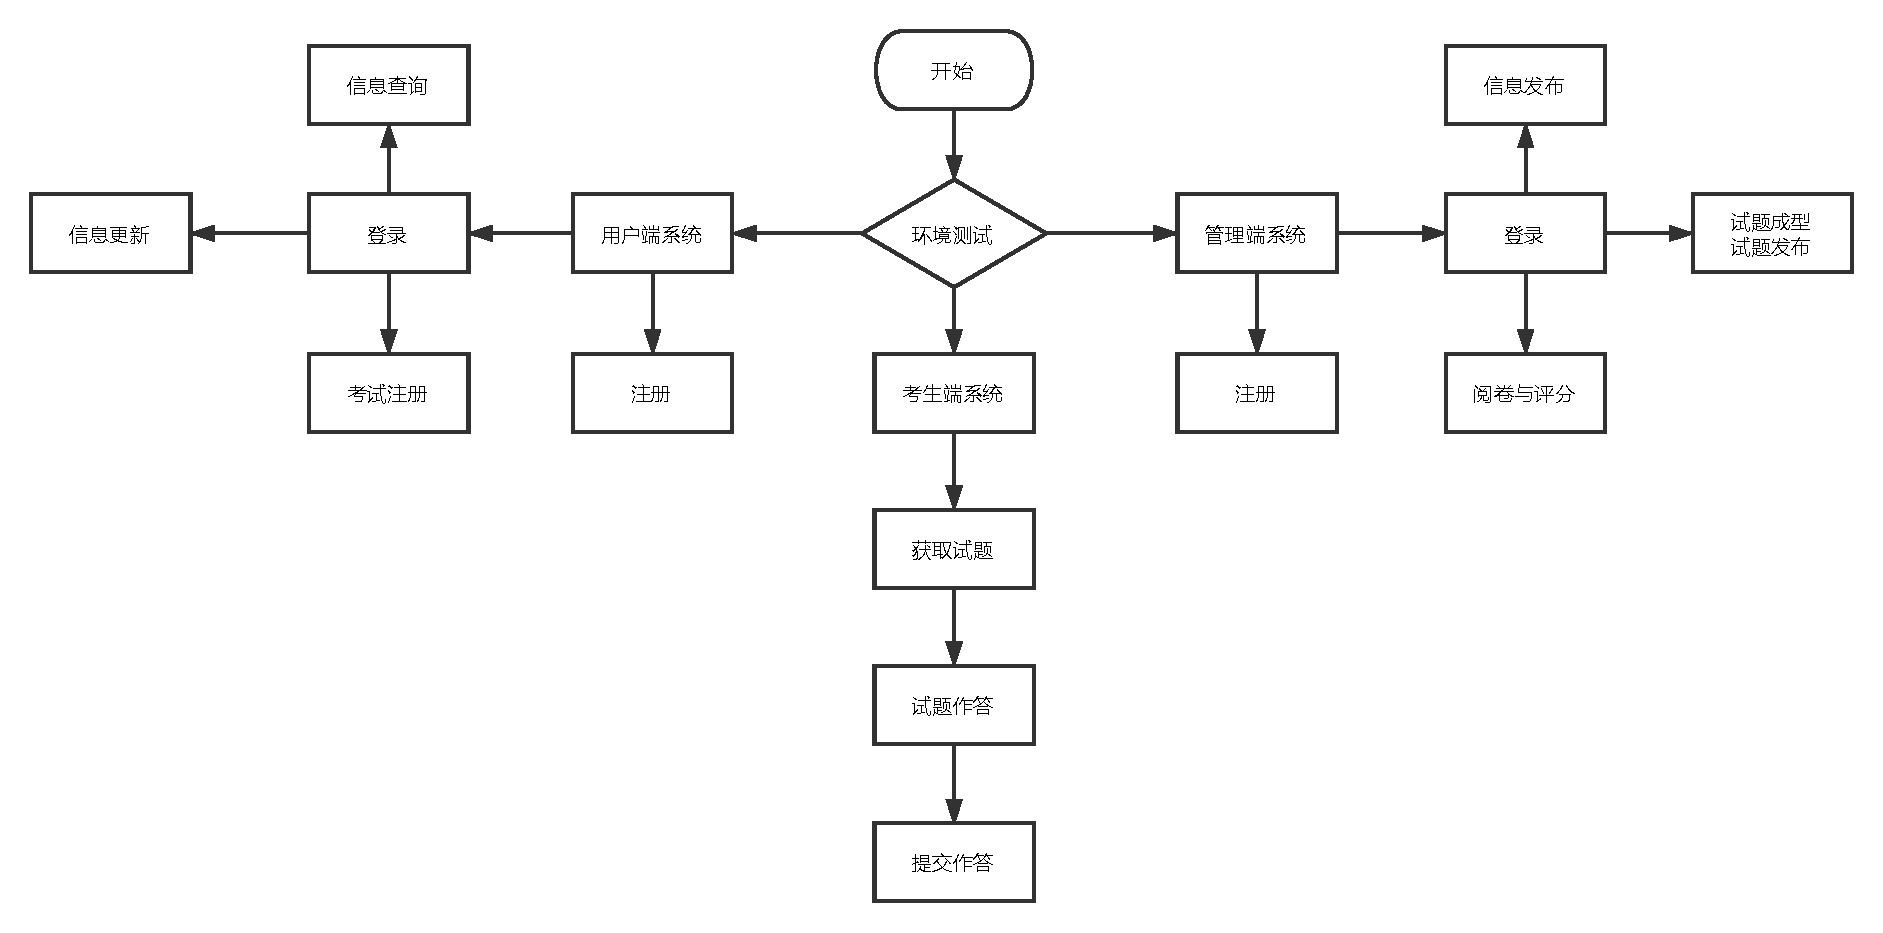
\includegraphics[width=10cm]{basic}
\caption{注册功能具体流程} \label{fig:figure1}
\end{figure}

用户向ETS系统发送注册请求后,ETS系统返回给用户具体的表单信息,用户根据提示,完善其用户名、密码、真实姓名、生日、身份证号、地址等信息,然后将表单提交给ETS系统,ETS系统根据用户提供的个人信息,检索其注册用户库,若发现重复,其生成新用户失败,返回提示信息,告知用户已存在相关账户,提示用户直接登录,否则,在数据库中录入用户个人信息,并告知用户已经注册成功,然后转入登录流程。

\subsection{登录功能具体流程}
\begin{figure}[ht]
\centering
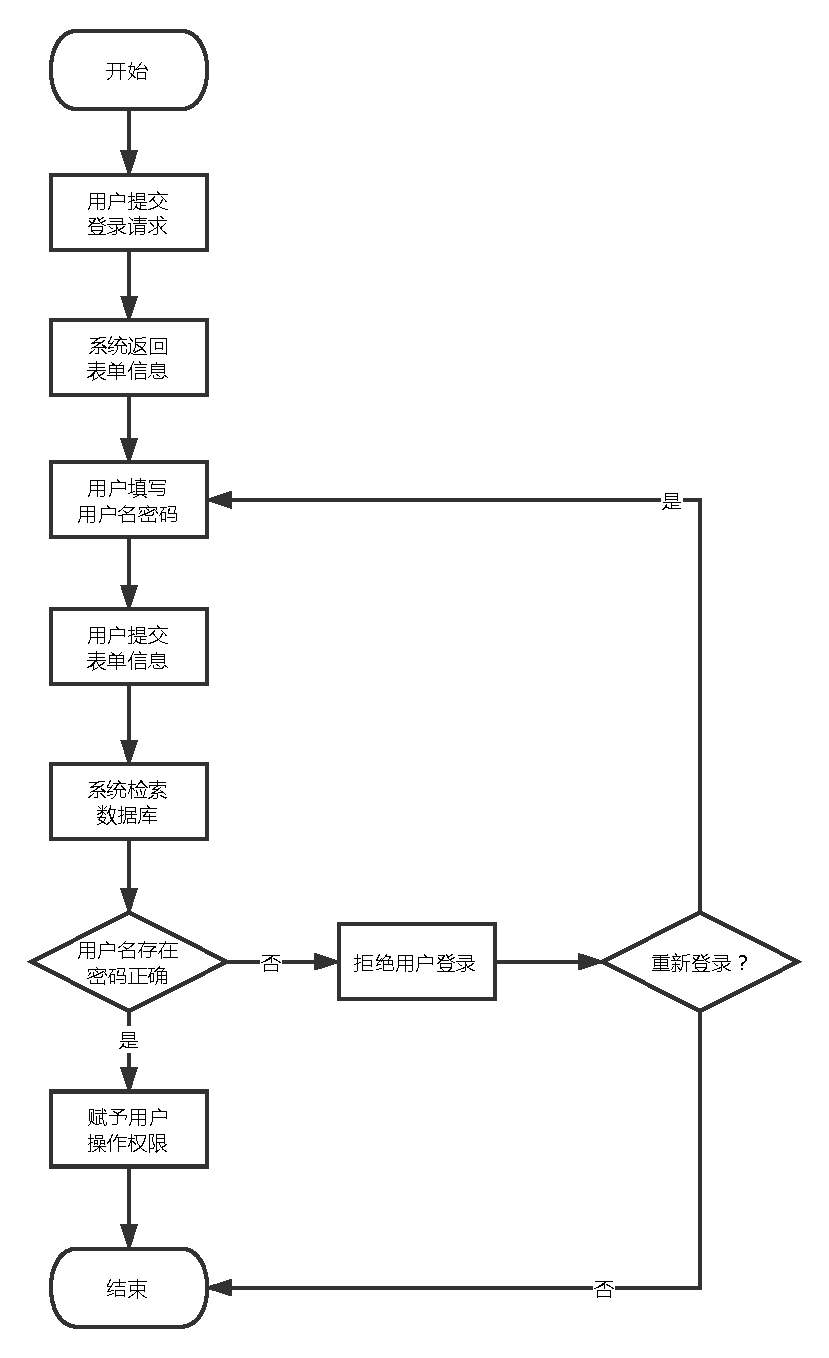
\includegraphics[width=10cm]{login}
\caption{登录功能具体流程} \label{fig:figure1}
\end{figure}

用户向ETS系统发送登录请求,ETS系统返回给用户具体的表单,要求用户输入其用户名和密码,用户输入完毕后,提交该表单信息,ETS系统根据表单信息检索数据库,若用户名存在,且密码与该用户名匹配,则返回给用户操作更多流程的权限,否则拒绝用户的进一步访问,要求用户重新提交用户名和密码。

\subsection{个人信息查询功能具体流程}
\begin{figure}[ht]
\centering
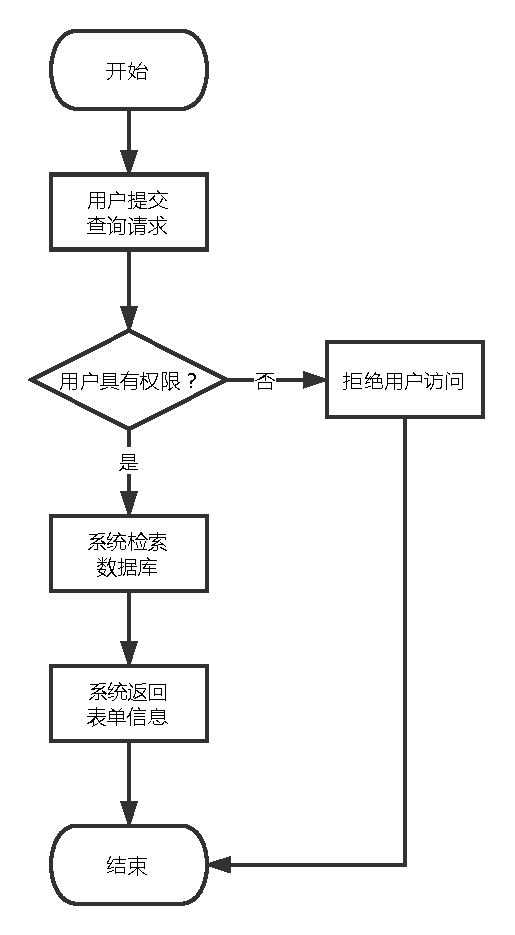
\includegraphics[width=10cm]{personal_info}
\caption{个人功能具体流程} \label{fig:figure1}
\end{figure}

用户向ETS系统发送查询请求,并指明查询的具体信息,ETS系统在接收到查询请求后,检查用户是否具有相应的查询权限,若有,则检索数据库系统,并返回相应的信息,否则返回提示信息,告知用户因权限不足访问被拒绝。

\subsection{考试信息发布功能具体流程}
\begin{figure}[ht]
\centering
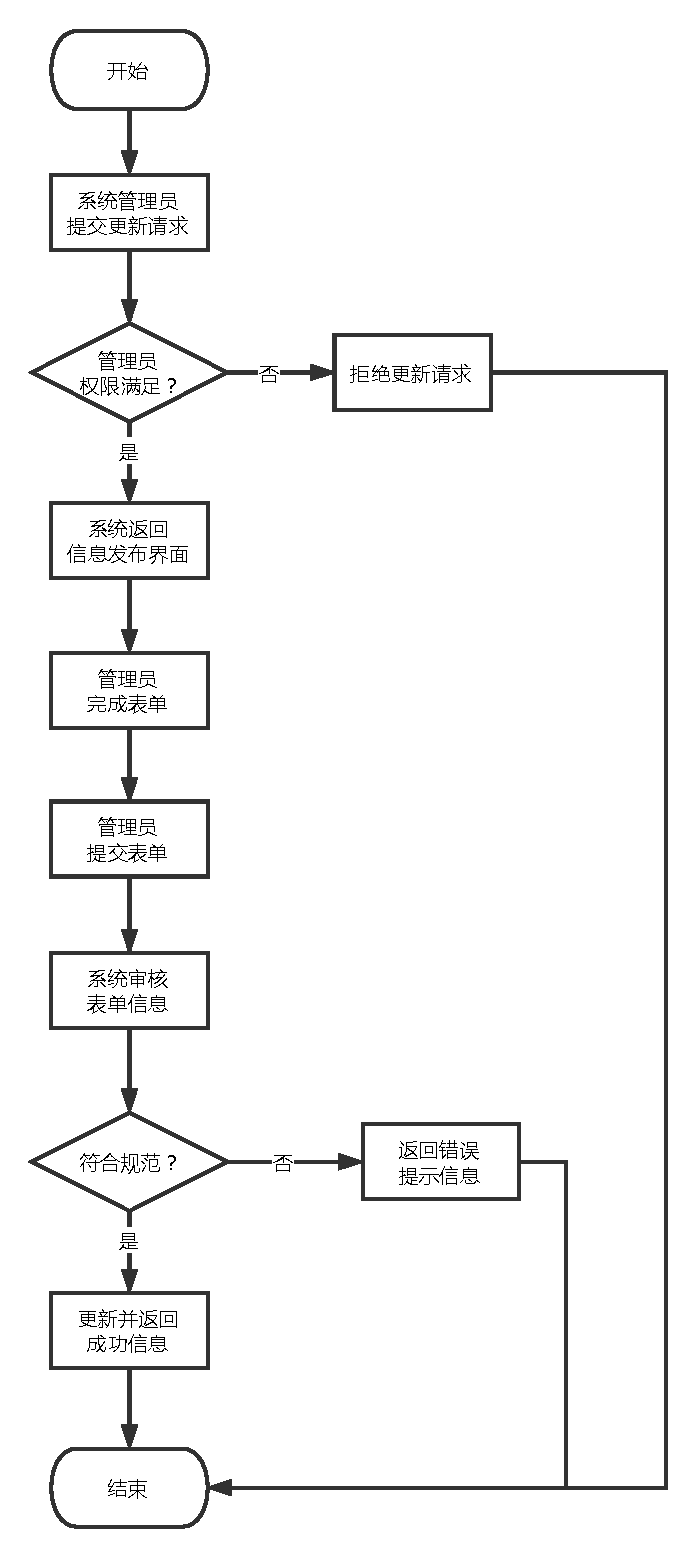
\includegraphics[width=10cm]{exam_info}
\caption{考试信息发布功能具体流程} \label{fig:figure1}
\end{figure}

ETS系统管理员向ETS系统发送考试信息更新请求,ETS系统在接收到请求后,检查ETS系统管理员的具体权限,若权限满足要求,则返回给ETS管理员发布考试信息的界面,否则拒绝其请求。ETS管理员在获取发布界面后,按照固定的程式,填写好考试相关信息,再提交ETS系统审核,ETS系统将根据已存在高级规则,对ETS管理员添加的考试信息进行查验,若满足相关发布规则,则更新其数据库,否则返回错误信息,要求ETS管理员对信息进行更正。

\subsection{试题成型功能具体流程}
\begin{figure}[ht]
\centering
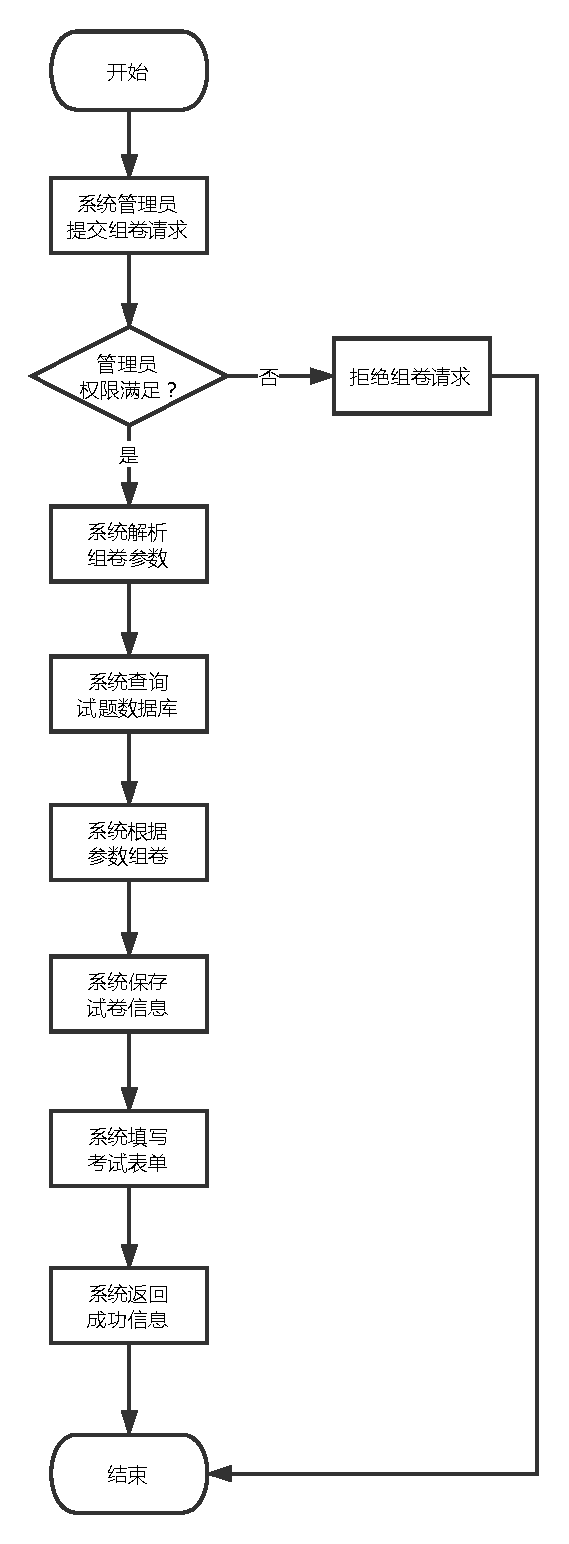
\includegraphics[width=8cm]{paper}
\caption{试题成型功能具体流程} \label{fig:figure1}
\end{figure}

ETS系统管理员向ETS系统发送组卷请求,并在该请求中,附带部分组卷参数,ETS系统在接收到请求后,解析组卷参数,然后查询数据库,按照参数所指定的组卷算法,生成一套试题,并将试题代号添加进与考试日期相关的表单中,然后返回成功信息,告知ETS管理员组卷成功。

\subsection{试卷分发与测试功能具体流程}
\begin{figure}[ht]
\centering
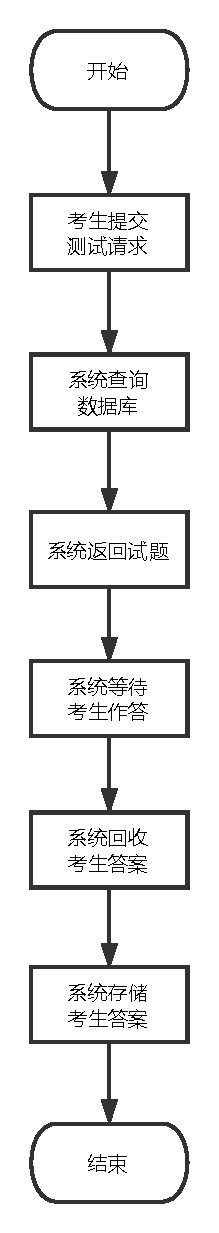
\includegraphics[width=4cm]{test}
\caption{试卷分发与测试功能具体流程} \label{fig:figure1}
\end{figure}

考生在考试界面上,向ETS系统发送测试请求,ETS以日期为关键字定位到具体考试,并检索该场考试的表单信息,提取试卷代号,然后在数据库中根据代号提取出完整试题,然后返回给考生测试的客户端界面,在考生测试完毕后,ETS系统接收到考生的提交请求,然后存储考生的作答信息,留待后续阅卷流程进行操作。

\subsection{试卷批改功能具体流程}
\begin{figure}[ht]
\centering
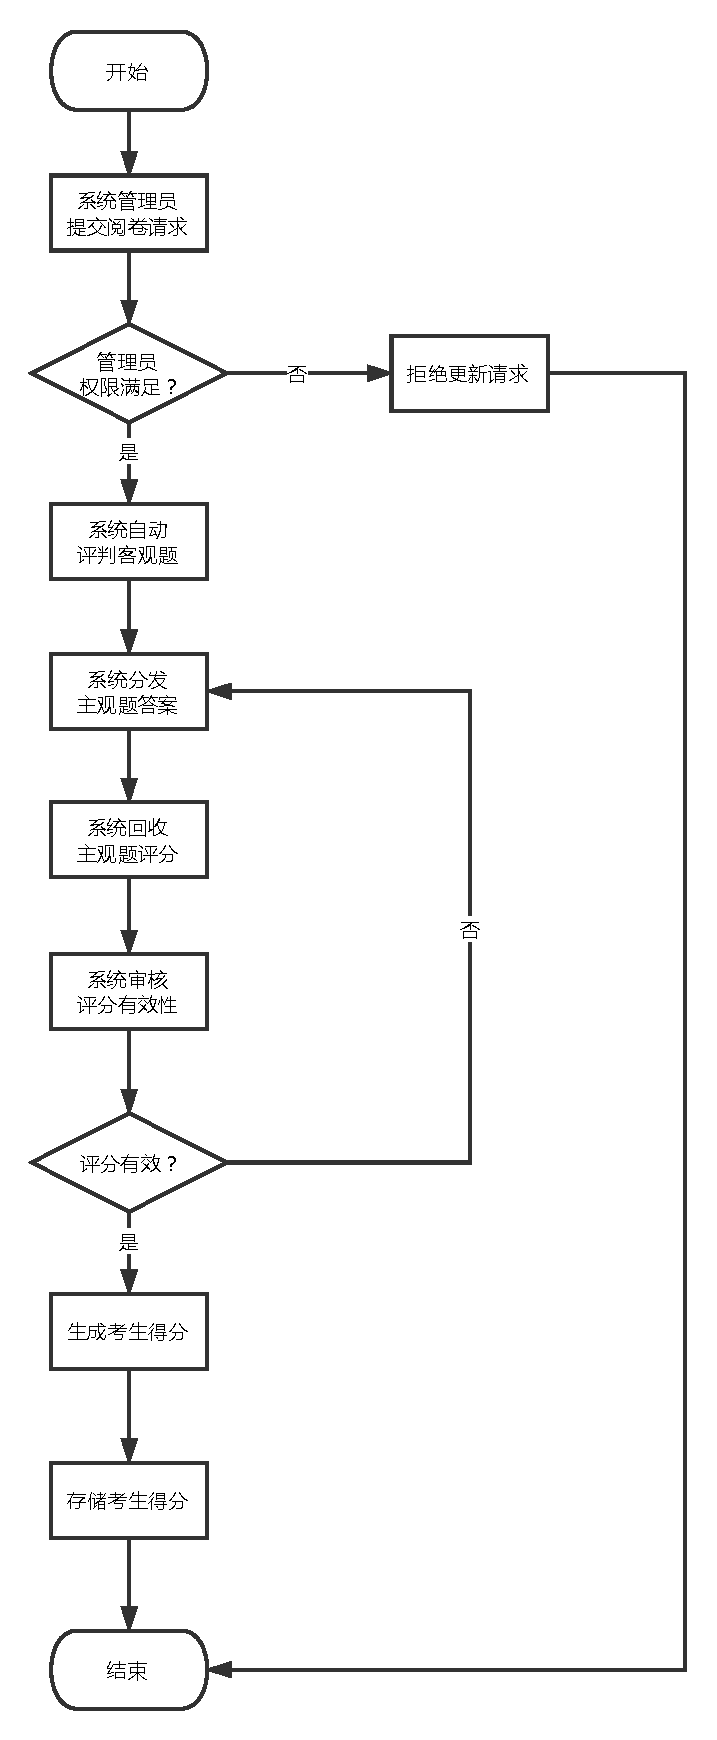
\includegraphics[width=10cm]{grading}
\caption{试卷批改功能具体流程} \label{fig:figure1}
\end{figure}

ETS管理员向ETS系统发送阅卷请求,ETS系统提取考生的客观题答题信息,与标准答案进行匹配,自动生成客观题部分的评分,之后,提取用户考生的主观题答题信息,根据ETS管理员所请求的参数,将考生答案提交给多位阅卷者,其中每位考生的每个答案,将同时提交给两位阅卷者,然后等待阅卷者返回分数信息。若阅卷者返回的同一考生的同一个作答的分数差异较大,则ETS系统将其提交给第三位权威阅卷者,否则则取其平均分作为考生该项目得分。


\section{功能结构设计}
\subsection{整体结构}
系统整体上分成两个模块,分别是考生用户子系统和ETS管理子系统。考生用户子系统处理考生用户提交的各类请求,ETS管理系统则提供更大权限,除了提供ETS方面提交的请求外,还可以对整个数据库有操作权限。

\subsection{用户端结构}
用户端特指考生用户子系统。它可以根据提供的服务划分不同的模块,包括用户注册模块、个人信息查询与更新模块、考试信息查询模块、考试报名模块、成绩查询模块等。它们之间没有耦合关系。

\subsection{服务器端结构}
服务器端特指ETS管理子系统。它也可以按照不同的服务划分不同的模块,包括考试信息发布、试题成型、试卷分发及测试、试卷批改各模块。其中,试卷批改模块依赖于试卷分发及测试模块,而试卷分发及测试模块依赖于试题成型模块。



\section{功能需求与程序代码的关系}
[此处指的是不同的需求分配到哪些模块去实现。可按不同的端拆分此表]
\begin{table}[htbp]
\centering
\caption{功能需求与程序代码的关系表} \label{tab:requirement-module}
\begin{tabular}{|c|c|c|}
    \hline
    · & 考生用户子系统 & ETS管理系统 \\
    \hline
    用户注册 & Y & · \\
    \hline
    个人信息查询与修改 & Y & · \\
    \hline
    考试信息查询 & Y & · \\
    \hline
    考试报名 & Y & · \\
    \hline
    成绩查询 & Y & · \\
    \hline
    考试信息发布 & · & Y \\
    \hline
    试题成型 & · & Y \\
    \hline
    试卷分发及测试 & · & Y \\
    \hline
    试卷批改 & · & Y \\
    \hline
\end{tabular}
\note{各项功能需求的实现与各个程序模块的分配关系}
\end{table}
\chapter{接口设计}
\section{外部接口}
比如说需要用到支付宝等外部支付系统,接口应当如何封装。

\subsection{支付宝接口}
详细讲述不同的接口(查询状态、支付交易、获取回执等)

\section{内部接口}
内部模块/系统之间的交互的接口。
\chapter{数据结构设计}
\section{逻辑结构设计}
\subsection{数据结构设计}
本章节主要描述程序运行逻辑中,除了数据库部分外,还需要额外使用的数据结构。

由于ETS考试管理系统的本质为客户端—服务器系统,其中客户端为用户进行注册、登录、信息查询、更新等操作的系统,服务器端为管理员进行信息发布、试题添加、试题成型、阅卷评分的操作的系统,故本章在数据结构的描述上将分客户端数据结构与服务器端数据结构进行。

\subsection{客户端数据结构}
1、存储用户个人信息的结构体,其域包括:用户名、密码、真实姓名、生日、身份证号、电子邮箱、联系电话、联系地址等,通过该结构体,客户端能及时记录下用户注册所填写的个人信息,之后再通过表单的形式发送给服务器端,从而更新服务器端的数据库

2、存储用户查询信息的结构体,其域包括:查询指令、查询参数等,通过该结构体,客户端能及时记录下用户希望查询的信息,之后可通过表单的形式发送给服务器端,从而获取服务器端的响应

3、存储用户试题作答情况的索引数组,其存储用户作答时每个答案存储的地址,在提交答案时,需要将该索引数组与存储的所有答案一并提交给服务器端,服务器端通过对索引数组的解析,从答案集中分离出各个题目的答案,然后存入数据库中,留待阅卷评分阶段对其进行操作

\subsection{服务器端数据结构}
1、大量数据库表,存储系统运行所必须的信息

2、优先队列,实现对所有学生成绩的动态排序,从而能够生成考生考试情况的位次信息,位次信息作为反馈信息的一部分,能够用来宏观调控最终的考生成绩,从而保证在不同试题难度下,分数能够做到相对客观

3、普通队列,存储所有请求,从而保证能够依次对各个请求进行处理

\section{物理结构设计}
各数据结构无特殊物理结构要求。

\section{数据结构与程序模块的关系}
[此处指的是不同的数据结构分配到哪些模块去实现。可按不同的端拆分此表]
\begin{table}[htbp]
\centering
\caption{数据结构与程序代码的关系表} \label{tab:datastructure-module}
\begin{tabular}{|c|c|c|}
    \hline
    · & 考生用户子系统 & ETS管理子系统 \\
    \hline
    用户信息结构体 & Y & · \\
    \hline
    考生用户查询信息结构体 & Y & · \\
    \hline
    ETS管理员查询信息结构体 & · & Y \\
    \hline
    试题索引数组 & · & Y \\
    \hline
    优先队列 & · & Y \\
    \hline
    普通队列 & Y & · \\
    \hline
\end{tabular}
\note{各项数据结构的实现与各个程序模块的分配关系}
\end{table}
\chapter{数据库设计}
\section{数据库环境说明}
本系统的数据系统采用Oracle数据库系统。


\section{数据库的命名规则}
是否允许单词缩写,允许的单词缩写有哪些。

表名是单数还是复数。关联表如何命名。字符数限制等。

字段是否带上前缀(如integer类型则加上i前缀等)。

\section{逻辑设计}
数据库应达到3NF范式。以新奥尔良方法为基础,基于ER模型和关系模式进行数据库设计。

概念设计:基于ER模型。

逻辑设计:基于关系模式设计。

采用的计算机辅助设计工具:PowerDesigner(SYBASE)。

\subsection{ER模型要素}

\subsubsection{实体}
本应用数据库中涉及到的实体有:考生、考试、试卷。

\subsubsection{联系}
实体与实体间的联系有:

1、考生与考试间的报名关系,是一个多对多的关系。

2、考生与考试间的参加关系,是一个多对多的关系。

3、考试与试卷间的使用关系,是一个多对一的关系。

\subsubsection{确定实体属性}
考生具有的属性有:姓名、性别、生日、证件号、地区、邮寄地址、联系方式。其中证件号是主码。

考试具有的属性有:时间、地点。(时间,地点)是主码。

试卷具有的属性有:试卷编号,题1编号,...,题100编号。试卷编号是主码。

\subsubsection{确定联系属性}
考生和考试间的参加关系具有“成绩”属性。

\section{示例}
\begin{figure}[ht]
\centering
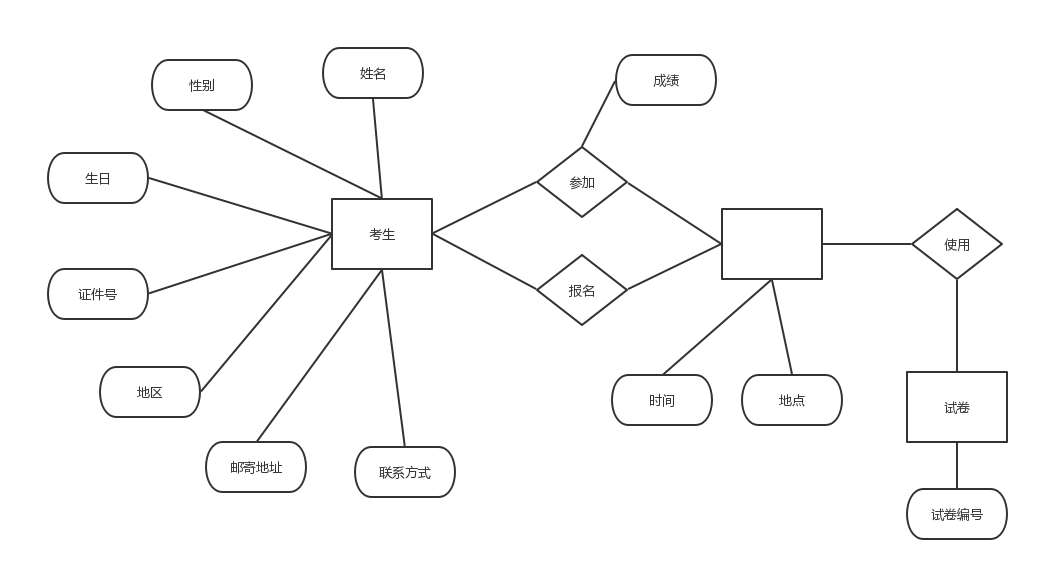
\includegraphics[width=16cm]{ER.png}
\caption{ER图} \label{fig:figure1}
\end{figure}



\section{物理设计}

\subsection{数据库产品}
使用 Oracle Database 12c 企业版,采用集中式的数据库。

\subsection{实体属性、类型、精度}
考生、考试、试卷三个实体各自转换成一个关系模式。除此以外,由于考生与考试间的报名关系、考生与考试间的参加关系是多对多的关系,因此也要各转换成一个关系模式。
\subsubsection{考生数据表Examinee设计}
\begin{table}[htbp]
\centering
\caption{考生数据表Examinee设计} \label{tab:client-database}
\begin{tabular}{|c|c|c|c|c|}
    \hline
    字段名 & 类型 & 大小 & 说明 & 备注 \\
    \hline
    name & char & 20 & 用户的英文姓名 & · \\
    \hline
    sex & char & 1 & 用户的性别 & · \\
    \hline
    date of birth & date & · & 用户的生日 & · \\
    \hline
    ID & char & 64 & 用户的证件号 & 主码 \\
    \hline
    location & char & 200 & 用户所在地区(大范围) & · \\
    \hline
    mail address & char & 200 & 用户希望的成绩单邮寄地址 & · \\
    \hline
    contact & char & 11 & 用户的手机号或电话号 & · \\
    \hline
\end{tabular}
\note{考生数据表Examinee设计}
\end{table}

\subsubsection{考试数据表Exam设计}
记录未来12月将举办的考试的时间、考点与考位信息。
\begin{table}[htbp]
\centering
\caption{考试数据表Exam设计} \label{tab:order-database}
\begin{tabular}{|c|c|c|c|c|}
    \hline
    字段名 & 类型 & 大小 & 说明 & 备注 \\
    \hline
    time & date & · & 考试的日期 & 和centerNo一起构成主码 \\
    \hline
    centerNo & int & 4 & 举办考试的考点编号 & 和time一起构成主码 \\
    \hline
    quota & int & 4 & 剩余考位 & · \\
    \hline
\end{tabular}
\note{考试数据表Exam设计}
\end{table}

\subsubsection{试卷数据表设计}
试卷数据表中记录每份试卷的题目在题库中的编号。默认每份试卷有100题。每份试卷有唯一的编号,是整型。

\begin{table}[htbp]
\centering
\caption{试卷数据表TestPaper设计} \label{tab:order-database}
\begin{tabular}{|c|c|c|c|c|}
    \hline
    字段名 & 类型 & 大小 & 说明 & 备注 \\
    \hline
    paperNo & int & 4 & 试卷编号 & 主码 \\
    \hline
    Q1No & int & 4 & 第1题编号 & · \\
    \hline
    ... & ... & ... & ... & ... \\
    \hline
    Q100No & int & 4 & 第100题编号 & · \\
    \hline
\end{tabular}
\note{试卷数据表TestPaper设计}
\end{table}

\subsubsection{考试注册数据表Registration设计}
该表只记录尚未举行的考试的报名信息。
\begin{table}[htbp]
\centering
\caption{考试注册数据表Registration设计} \label{tab:order-database}
\begin{tabular}{|c|c|c|c|c|}
    \hline
    字段名 & 类型 & 大小 & 说明 & 备注 \\
    \hline
    examineeID & char & 64 & 考生的证件号 & 和centerNo一起构成主码 \\
    \hline
    examTime & date & · & 考试日期 & 和examineeID、centerNo一起构成主码 \\
    \hline
    centerNo & int & 4 & 举办考试的考点编号 & 和examineeID、examTime一起构成主码 \\
    \hline
\end{tabular}
\note{考试注册数据表Registration设计}
\end{table}

\subsubsection{考生考试成绩数据表Grades设计}
\begin{table}[htbp]
\centering
\caption{考生考试成绩数据表Grades设计} \label{tab:order-database}
\begin{tabular}{|c|c|c|c|c|}
    \hline
    字段名 & 类型 & 大小 & 说明 & 备注 \\
    \hline
    examineeID & char & 64 & 考生的证件号 & 和examTime、centerNo一起构成主码,同时是外码 \\
    \hline
    examTime & date & · & 考试日期 & 和examineeID、centerNo一起构成主码,同时是外码 \\
    \hline
    centerNo & int & 4 & 举办考试的考点编号 & 和examineeID、examTime一起构成主码,同时是外码 \\
    \hline
    grade & int & 4 & 考生成绩 & · \\
    \hline
\end{tabular}
\note{考生考试成绩数据表Grades设计}
\end{table}



\section{安全性设计}
备份和容灾设计。

服务器中的数据需定期备份。其中,考生用户的数据每小时备份一次,考试注册信息每小时备份一次。试卷与题库数据在每次更新时备份一次,考生成绩数据在每举行一次考试以及出分时各备份一次。考试信息一般不发生变化,因此除非有更新,否则一个月备份一次。

服务器必须安装不间断电源以防止停电或电压不稳造成的数据丢失的损失。若真断电时,在断电恢复过程可采用Oracle的日志文件,对其进行ROLLBACK处理,对数据进行恢复。

此外,服务器应在多个地方有冗余存储,如在多个城市建立数据中心进行数据的冗余备份,以防遭受人为或自然的破坏。

\section{数据库管理与维护说明}
对于数据库的维护,随时对数据库中的信息加以调试和保存备份。同样需要个工作人员进行系统的分析和用户的反馈,对系统进行升级以及功能的完善。同时保证系统安全有序的运行。

数据库的维护工作由ETS的专门管理人员完成。主要的维护工作有:

1、为各个数据表建立适当的索引以加快查询

2、定期(一般为一个月)发布新的考试信息

3、发布新试题时更新testPaper数据表信息

4、在每次考试后,将数据从Registration表中迁移到Grades表中,并加上考生成绩属性

5、定期(一般为一个月)将数据备份至永久存储介质(如磁带等)

6、对各类用户授予合适的权限

6、为数据建立完整性约束,如类型约束、引用完整性约束等。
\chapter{界面设计}
\section{客户端界面}
A. 对于用户注册与管理系统的用户接口说明如下,这一部分对应于功能需求中新用户注册、个人信息查询与修改、查询考试信息以及预缴费的部分:

\begin{figure}[ht]
\centering
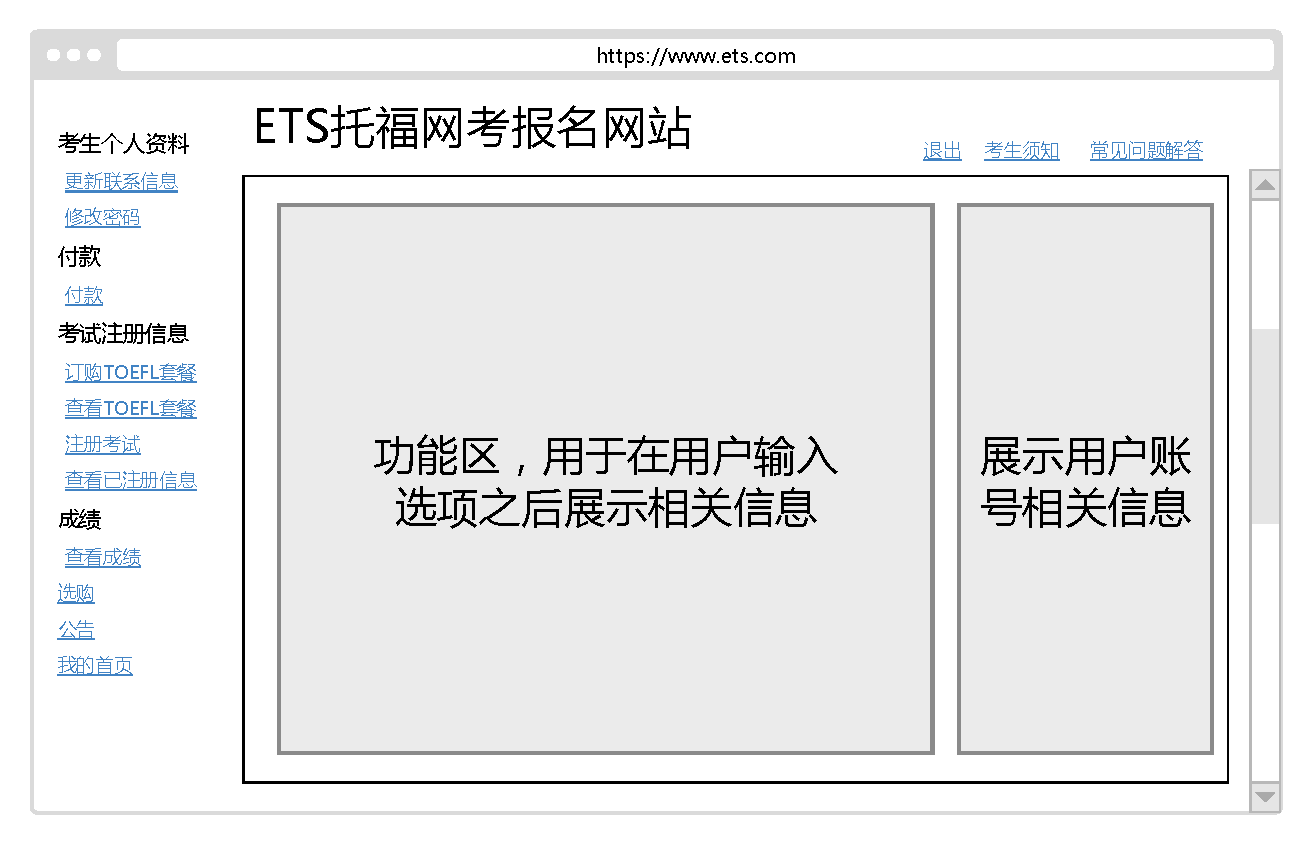
\includegraphics[width=10cm]{UI}
\caption{用户接口A}\label{fig:noted-figure}
%\note{the solid lines represent the time histogram of the spontaneous activities of an old monkey cell(gray) and a young monkey cell (black). The bin-width is 1}
\end{figure}

用户使用浏览器输入网址***.org后进入登录界面。输入ID和密码即可登录。在登录框下部提供两个按键“新用户注册”和“密码找回”。

用户点击“新用户注册”按键后,进入注册界面,其中包括各个文本框与下拉框供用户输入信息,所需输入的信息已在3.1节详细说明。

用户点击“密码找回”按键后,进入验证界面,可以选择邮箱验证或手机验证。通过注册时所填的邮箱或手机可以得到验证码,用户输入正确的验证码后,可以设置新密码。

当用户成功登录后,将进入个人中心界面,其中提供了各个功能板块,每个里面包括了一组相似功能的按键。

1、个人资料:提供“更新联系信息”和“修改密码”的按键;
	
2、考试记录:提供“考位查询”、“全年考试时间与地点查询”、“注册考试”、“查看已注册考试”、“查看成绩”的按键;

3、余额:提供“预付款”的按键。

\section{服务器端界面}
B. 对于试题管理系统的用户接口说明如下,这一部分对应于功能需求中题库维护、试题成型和试卷批改的部分:

\begin{figure}[ht]
\centering
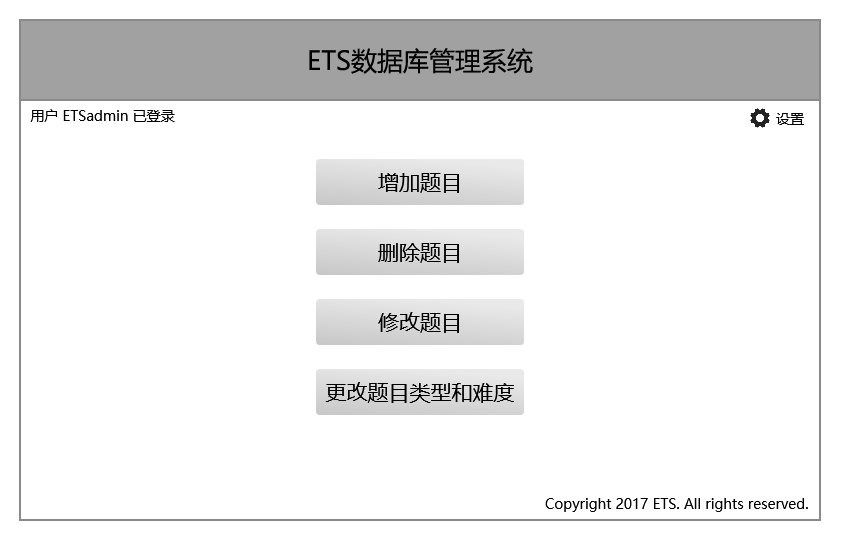
\includegraphics[width=10cm]{UI2.png}
\caption{用户接口B1}\label{fig:noted-figure}
%\note{the solid lines represent the time histogram of the spontaneous activities of an old monkey cell(gray) and a young monkey cell (black). The bin-width is 1}
\end{figure}

\begin{figure}[ht]
\centering
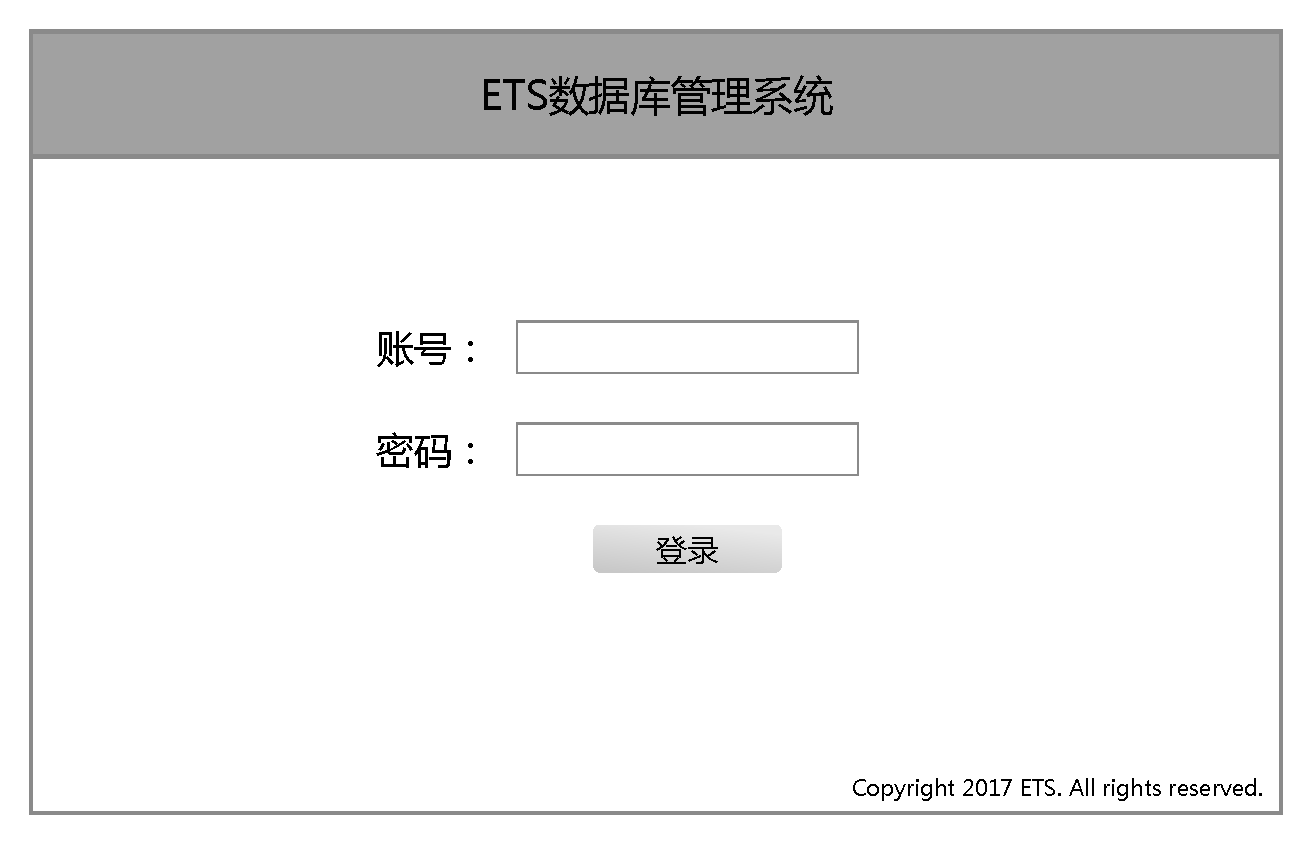
\includegraphics[width=10cm]{UI2-2}
\caption{用户接口B2}\label{fig:noted-figure}
%\note{the solid lines represent the time histogram of the spontaneous activities of an old monkey cell(gray) and a young monkey cell (black). The bin-width is 1}
\end{figure}

管理人员在服务器上运行指定的应用程序后进入登录界面,显示输入框要求输入账户和密码;登录成功后进入主界面,主界面的中央显示主菜单,菜单的选项同3.1中的说明相对应;右下角显示设置字样,点击后将能够查看设置并且进行修改。用户选择任意选项之后,主界面将按照3.1中的功能需求所对应的部分列出具体选项以及显示内容。

C. 对于考试系统的用户接口说明如下,这一部分对应于功能需求中试卷分发及测试的部分:

\begin{figure}[ht]
\centering
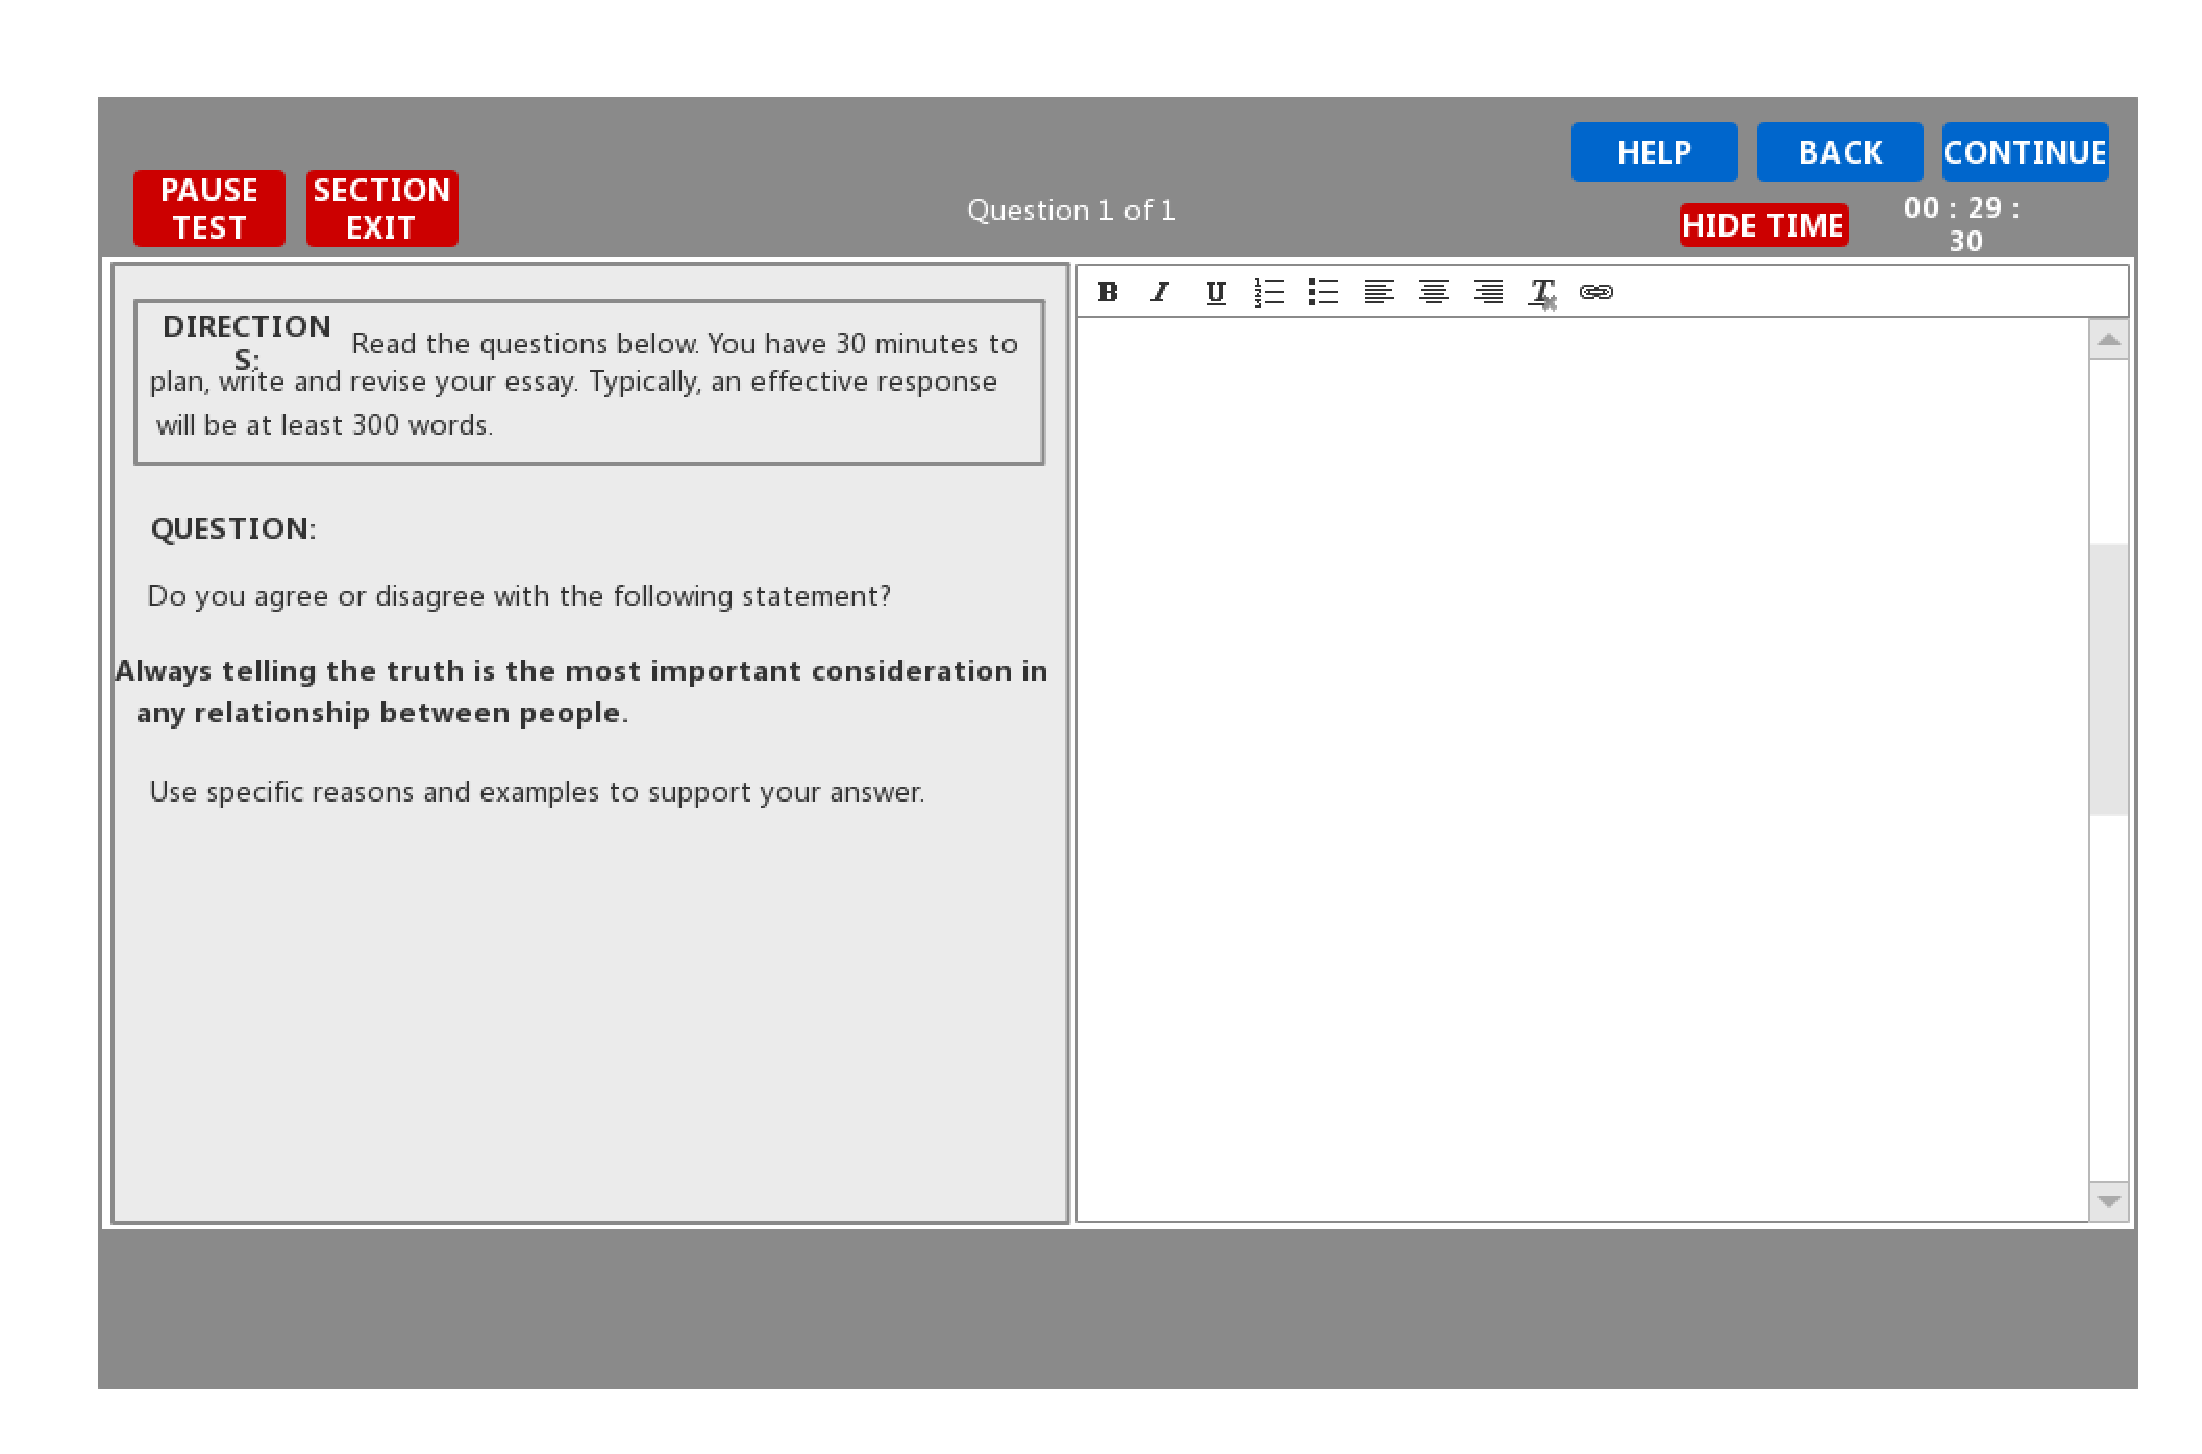
\includegraphics[width=15cm]{ETSwriting}
\caption{用户接口C1}\label{fig:noted-figure}
%\note{the solid lines represent the time histogram of the spontaneous activities of an old monkey cell(gray) and a young monkey cell (black). The bin-width is 1}
\end{figure}

\begin{figure}[ht]
\centering
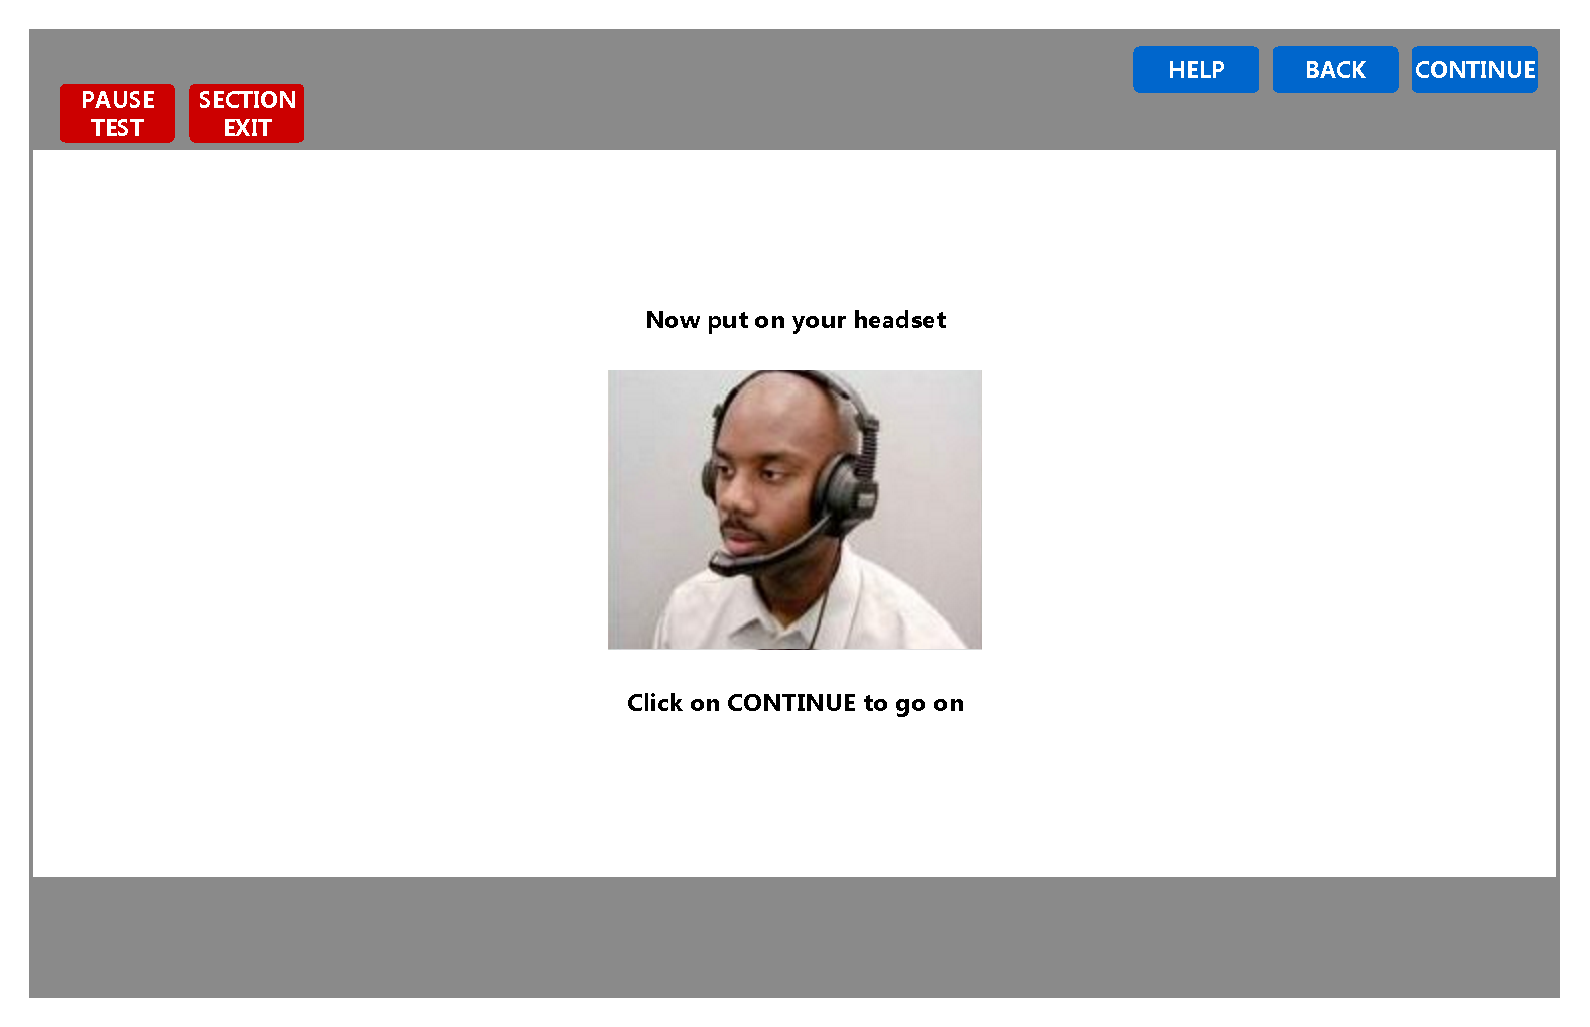
\includegraphics[width=15cm]{ETSlistening}
\caption{用户接口C2}\label{fig:noted-figure}
%\note{the solid lines represent the time histogram of the spontaneous activities of an old monkey cell(gray) and a young monkey cell (black). The bin-width is 1}
\end{figure}

用户将在考场给定的设备上使用本系统。考试未开始时,主界面将显示输入框,提示用户输入验证信息;

用户完成验证之后,主界面将显示用户的注册信息,直至考试开始;

考试开始之后,主界面将显示题目和对应的材料。用户能够根据鼠标点击来选择题目所对应的选项;主界面右上角提供调节音量、切换至下一题、切换回上一题、确认完成本部分的按钮,用户点击之后将触发相应的动作,该动作若当前不可触发应该显示为灰色;在按钮下方实时显示当前部分所剩余的时间,并且在时间的右侧显示“隐藏时间”的按钮,用户点击之后时间将被隐藏。

另外,在展示题目时,如果该部分材料需要和题目一同出现,那么将以页面的中轴线为界,在右侧显示材料,左侧显示相应的题目。对于阅读材料,用户应当能够利用鼠标滚轮上下移动材料。只显示题目时,题目应当显示在屏幕中央。

以上三部分都应具有友好的用户界面和使用提示,使得没有系统使用基础的用户不需要经过特定的培训就可以顺利使用本系统。

\chapter{出错处理设计}
\section{数据库出错处理}
多重备份时,应采取何种策略,先利用哪一份备份;系统是否暂停服务等。

\section{某模块失效处理}
是否整个系统暂停服务,还是维持最小服务状态、如何尽快恢复服务还是删库跑路等。
\chapter{安全保密设计}
可能的内容包括保密性、是否采取加密传输、密钥如何分发和管理等。

安全性设计:

1、身份验证:用户登录系统才能进行操作

2、数据限制:访问数据库用户的所属类别决定访问的数据范围及操作权限

3、功能限制:通过用户功能视图限制用户对数据的操作

考生用户与系统之间传输的信息涉及到用户的隐私信息,应当保密,因此采用加密传输。使用https协议实现加密功能。每个考生用户的可见数据范围只有与自身相关的数据,这可以通过如下方式实现:在考生用户的每个请求中附加该用户的ID,把该ID作为查询条件的一部分。

ETS管理员用户直接在服务器端操作,不存在网络传输问题。应为各级管理人员设立相应的读写权限,这通过由DBA授权实现。
\chapter{维护设计}
可能的内容包括数据库的日常备份、压缩、维护等。

\chapter{图片}
本章展示图片相关用法。

\section{示例}
\begin{figure}[ht]
\centering

\includegraphics[width=10cm]{ustc_logo_fig}
\caption{测试图片} \label{fig:figure1}
\end{figure}

\section{带图注的图}
\begin{figure}[ht]
\centering

\includegraphics[width=10cm]{ustc_logo_fig}
\caption{带图注的图片}\label{fig:noted-figure}
\note{the solid lines represent the time histogram of the spontaneous activities of an old monkey cell(gray) and a young monkey cell (black). The bin-width is 1}
\end{figure}

\chapter{表格}

\section{A Simple Table}
\begin{table}[htbp]
\centering
\caption{这里是表的标题} \label{tab:simpletable}
\begin{tabular}{|c|c|}
    \hline
    a & b \\
    \hline
    c & d \\
    \hline
\end{tabular}
\note{这里是表的注释}
\end{table}

\section{长表格}
\begin{longtable}{ccc}
% 首页表头
\caption[长表格演示]{长表格演示} \label{tab:longtable} \\
\toprule[1.5pt]
名称  & 说明 & 备注\\
\midrule[1pt]
\endfirsthead
% 续页表头
\caption[]{长表格演示(续)} \\
\toprule[1.5pt]
名称  & 说明 & 备注 \\
\midrule[1pt]
\endhead
% 首页表尾
\hline
\multicolumn{3}{r}{\small 续下页}
\endfoot
% 续页表尾
\bottomrule[1.5pt]
\endlastfoot

AAAAAAAAAAAA   &   BBBBBBBBBBB   &   CCCCCCCCCCCCCC   \\
AAAAAAAAAAAA   &   BBBBBBBBBBB   &   CCCCCCCCCCCCCC   \\
AAAAAAAAAAAA   &   BBBBBBBBBBB   &   CCCCCCCCCCCCCC   \\
AAAAAAAAAAAA   &   BBBBBBBBBBB   &   CCCCCCCCCCCCCC   \\
AAAAAAAAAAAA   &   BBBBBBBBBBB   &   CCCCCCCCCCCCCC   \\
AAAAAAAAAAAA   &   BBBBBBBBBBB   &   CCCCCCCCCCCCCC   \\
AAAAAAAAAAAA   &   BBBBBBBBBBB   &   CCCCCCCCCCCCCC   \\
AAAAAAAAAAAA   &   BBBBBBBBBBB   &   CCCCCCCCCCCCCC   \\
AAAAAAAAAAAA   &   BBBBBBBBBBB   &   CCCCCCCCCCCCCC   \\
AAAAAAAAAAAA   &   BBBBBBBBBBB   &   CCCCCCCCCCCCCC   \\
AAAAAAAAAAAA   &   BBBBBBBBBBB   &   CCCCCCCCCCCCCC   \\
AAAAAAAAAAAA   &   BBBBBBBBBBB   &   CCCCCCCCCCCCCC   \\
AAAAAAAAAAAA   &   BBBBBBBBBBB   &   CCCCCCCCCCCCCC   \\
AAAAAAAAAAAA   &   BBBBBBBBBBB   &   CCCCCCCCCCCCCC   \\
AAAAAAAAAAAA   &   BBBBBBBBBBB   &   CCCCCCCCCCCCCC   \\
AAAAAAAAAAAA   &   BBBBBBBBBBB   &   CCCCCCCCCCCCCC   \\
AAAAAAAAAAAA   &   BBBBBBBBBBB   &   CCCCCCCCCCCCCC   \\
AAAAAAAAAAAA   &   BBBBBBBBBBB   &   CCCCCCCCCCCCCC   \\
AAAAAAAAAAAA   &   BBBBBBBBBBB   &   CCCCCCCCCCCCCC   \\
AAAAAAAAAAAA   &   BBBBBBBBBBB   &   CCCCCCCCCCCCCC   \\
AAAAAAAAAAAA   &   BBBBBBBBBBB   &   CCCCCCCCCCCCCC   \\
AAAAAAAAAAAA   &   BBBBBBBBBBB   &   CCCCCCCCCCCCCC   \\
AAAAAAAAAAAA   &   BBBBBBBBBBB   &   CCCCCCCCCCCCCC   \\
AAAAAAAAAAAA   &   BBBBBBBBBBB   &   CCCCCCCCCCCCCC   \\
AAAAAAAAAAAA   &   BBBBBBBBBBB   &   CCCCCCCCCCCCCC   \\
AAAAAAAAAAAA   &   BBBBBBBBBBB   &   CCCCCCCCCCCCCC   \\
AAAAAAAAAAAA   &   BBBBBBBBBBB   &   CCCCCCCCCCCCCC   \\
AAAAAAAAAAAA   &   BBBBBBBBBBB   &   CCCCCCCCCCCCCC   \\
AAAAAAAAAAAA   &   BBBBBBBBBBB   &   CCCCCCCCCCCCCC   \\
AAAAAAAAAAAA   &   BBBBBBBBBBB   &   CCCCCCCCCCCCCC   \\
AAAAAAAAAAAA   &   BBBBBBBBBBB   &   CCCCCCCCCCCCCC   \\
AAAAAAAAAAAA   &   BBBBBBBBBBB   &   CCCCCCCCCCCCCC   \\
AAAAAAAAAAAA   &   BBBBBBBBBBB   &   CCCCCCCCCCCCCC   \\
AAAAAAAAAAAA   &   BBBBBBBBBBB   &   CCCCCCCCCCCCCC   \\
AAAAAAAAAAAA   &   BBBBBBBBBBB   &   CCCCCCCCCCCCCC   \\
AAAAAAAAAAAA   &   BBBBBBBBBBB   &   CCCCCCCCCCCCCC   \\
\end{longtable}

\chapter{算法环境}
模板中使用 \texttt{algorithm2e} 宏包实现算法环境。关于该宏包的具体用法,
请阅读宏包的官方文档。

\begin{algorithm}[htbp]
\SetAlgoLined
\KwData{this text}
\KwResult{how to write algorithm with \LaTeX2e }

initialization\;
\While{not at end of this document}{
    read current\;
    \eIf{understand}{
        go to next section\;
        current section becomes this one\;
    }{
        go back to the beginning of current section\;
    }
}
\caption{算法示例1}
\label{algo:algorithm1}
\end{algorithm}

\IncMargin{1em}
\begin{algorithm}
\SetKwData{Left}{left}\SetKwData{This}{this}\SetKwData{Up}{up}
\SetKwFunction{Union}{Union}\SetKwFunction{FindCompress}{FindCompress}
\SetKwInOut{Input}{input}\SetKwInOut{Output}{output}

\Input{A bitmap $Im$ of size $w\times l$}
\Output{A partition of the bitmap}
\BlankLine
\emph{special treatment of the first line}\;
\For{$i\leftarrow 2$ \KwTo $l$}{
    \emph{special treatment of the first element of line $i$}\;
    \For{$j\leftarrow 2$ \KwTo $w$}{\label{forins}
        \Left$\leftarrow$ \FindCompress{$Im[i,j-1]$}\;
        \Up$\leftarrow$ \FindCompress{$Im[i-1,]$}\;
        \This$\leftarrow$ \FindCompress{$Im[i,j]$}\;
        \If(\tcp*[h]{O(\Left,\This)==1}){\Left compatible with \This}{\label{lt}
            \lIf{\Left $<$ \This}{\Union{\Left,\This}}
            \lElse{\Union{\This,\Left}}
        }
        \If(\tcp*[f]{O(\Up,\This)==1}){\Up compatible with \This}{\label{ut}
        \lIf{\Up $<$ \This}{\Union{\Up,\This}}
        \tcp{\This is put under \Up to keep tree as flat as possible}\label{cmt}
        \lElse{\Union{\This,\Up}}\tcp*[h]{\This linked to \Up}\label{lelse}
        }
    }
    \lForEach{element $e$ of the line $i$}{\FindCompress{p}}
}
\caption{算法示例2}\label{algo_disjdecomp}
\label{alog:algorithm2}
\end{algorithm}\DecMargin{1em}

\chapter{代码环境}
模板中使用 \texttt{listings} 宏包实现代码环境。详细用法见宏包的官方说明文档。

以下是代码示例,可以在文中任意位置引用\autoref{first-code} 。
\begin{lstlisting}[language=C, caption=示例代码, label={code:first-code}]
#include <stdio.h>

int main( )
{
    printf("hello, world\n");
    return 0;
}
\end{lstlisting}

\chapter{引用文献标注}

\section{著者-出版年制标注法}

\noindent
\verb|\citestyle{ustcauthoryear}|
\citestyle{ustcauthoryear}

\noindent
\begin{tabular}{l@{\quad$\Rightarrow$\quad}l}
  \verb|\cite{knuth86a}| & \cite{knuth86a}\\
  \verb|\citet{knuth86a}| & \citet{knuth86a}\\
  \verb|\citet[chap.~2]{knuth86a}| & \citet[chap.~2]{knuth86a}\\[0.5ex]
  \verb|\citep{knuth86a}| & \citep{knuth86a}\\
  \verb|\citep[chap.~2]{knuth86a}| & \citep[chap.~2]{knuth86a}\\
  \verb|\citep[see][]{knuth86a}| & \citep[see][]{knuth86a}\\
  \verb|\citep[see][chap.~2]{knuth86a}| & \citep[see][chap.~2]{knuth86a}\\[0.5ex]
  \verb|\citet*{knuth86a}| & \citet*{knuth86a}\\
  \verb|\citep*{knuth86a}| & \citep*{knuth86a}\\
\end{tabular}

\noindent
\begin{tabular}{l@{\quad$\Rightarrow$\quad}l}
  \verb|\citet{knuth86a,tlc2}| & \citet{knuth86a,tlc2}\\
  \verb|\citep{knuth86a,tlc2}| & \citep{knuth86a,tlc2}\\
  \verb|\cite{knuth86a,knuth84}| & \cite{knuth86a,knuth84}\\
  \verb|\citet{knuth86a,knuth84}| & \citet{knuth86a,knuth84}\\
  \verb|\citep{knuth86a,knuth84}| & \citep{knuth86a,knuth84}\\
\end{tabular}

\section{顺序编码制标注法}

\noindent
\verb|\citestyle{ustcnumerical}|
\citestyle{ustcnumerical}

\noindent
\begin{tabular}{l@{\quad$\Rightarrow$\quad}l}
  \verb|\cite{knuth86a}| & \cite{knuth86a}\\
  \verb|\citet{knuth86a}| & \citet{knuth86a}\\
  \verb|\citet[chap.~2]{knuth86a}| & \citet[chap.~2]{knuth86a}\\[0.5ex]
  \verb|\citep{knuth86a}| & \citep{knuth86a}\\
  \verb|\citep[chap.~2]{knuth86a}| & \citep[chap.~2]{knuth86a}\\
  \verb|\citep[see][]{knuth86a}| & \citep[see][]{knuth86a}\\
  \verb|\citep[see][chap.~2]{knuth86a}| & \citep[see][chap.~2]{knuth86a}\\[0.5ex]
  \verb|\citet*{knuth86a}| & \citet*{knuth86a}\\
  \verb|\citep*{knuth86a}| & \citep*{knuth86a}\\
\end{tabular}

\noindent
\begin{tabular}{l@{\quad$\Rightarrow$\quad}l}
  \verb|\citet{knuth86a,tlc2}| & \citet{knuth86a,tlc2}\\
  \verb|\citep{knuth86a,tlc2}| & \citep{knuth86a,tlc2}\\
  \verb|\cite{knuth86a,knuth84}| & \cite{knuth86a,knuth84}\\
  \verb|\citet{knuth86a,knuth84}| & \citet{knuth86a,knuth84}\\
  \verb|\citep{knuth86a,knuth84}| & \citep{knuth86a,knuth84}\\
  \verb|\cite{knuth86a,knuth84,tlc2}| & \cite{knuth86a,knuth84,tlc2}\\
\end{tabular}

\section{其他形式的标注}

\noindent
\begin{tabular}{l@{\quad$\Rightarrow$\quad}l}
  \verb|\citealt{tlc2}| & \citealt{tlc2}\\
  \verb|\citealt*{tlc2}| & \citealt*{tlc2}\\
  \verb|\citealp{tlc2}| & \citealp{tlc2}\\
  \verb|\citealp*{tlc2}| & \citealp*{tlc2}\\
  \verb|\citealp{tlc2,knuth86a}| & \citealp{tlc2,knuth86a}\\
  \verb|\citealp[pg.~32]{tlc2}| & \citealp[pg.~32]{tlc2}\\
  \verb|\citenum{tlc2}| & \citenum{tlc2}\\
  \verb|\citetext{priv.\ comm.}| & \citetext{priv.\ comm.}\\
\end{tabular}

\noindent
\begin{tabular}{l@{\quad$\Rightarrow$\quad}l}
  \verb|\citeauthor{tlc2}| & \citeauthor{tlc2}\\
  \verb|\citeauthor*{tlc2}| & \citeauthor*{tlc2}\\
  \verb|\citeyear{tlc2}| & \citeyear{tlc2}\\
  \verb|\citeyearpar{tlc2}| & \citeyearpar{tlc2}\\
\end{tabular}

\bibliography{bib/tex}


\end{document}
